% Latex template: mahmoud.s.fahmy@students.kasralainy.edu.eg
% For more details: https://www.sharelatex.com/learn/Beamer

\documentclass[aspectratio=169]{beamer}					% Document class

\usepackage[english]{babel}				% Set language
\usepackage[utf8x]{inputenc}			% Set encoding
\usepackage{latexsym}
\usepackage{amsmath}
\usepackage{booktabs}
\usepackage{url}
\usepackage{pgfplots}
\usepackage{pgfplotstable}
\usepackage{booktabs}
\usepackage{array}
\usepackage{colortbl}
\usepackage{filecontents}
\usetikzlibrary{patterns}
\usetikzlibrary{calc,positioning}
\usepgfplotslibrary{statistics}
\usepgfplotslibrary{groupplots}
\usepackage{tikzsymbols}
\usepackage{multicol}
\usepackage{ulem}
\usepackage{pdfpages}
%\usepackage{paralist}
%\usepackage{enumitem}
%\setlist{noitemsep}
\usepackage{tikz}
\usetikzlibrary{calc, shapes, backgrounds}
\usepackage{amsmath, amssymb}
\usepackage{listings}
  
\pgfplotsset{compat=1.12}

\newcommand{\todo}[1]{\textcolor{red}{#1}}
\newcommand{\dotn}[3]{\mathrm{dot^{\prime}_{#1}}(#2, #3)}
\newcommand{\quant}[1]{\mathrm{q}(#1)}
\newcommand{\Trans}[1]{#1^\mathrm{T}}
\newcommand{\dotint}[2]{#1 \times \Trans{#2}}

\definecolor{bblue}{HTML}{4F81BD}
\definecolor{rred}{HTML}{C0504D}
\definecolor{ggreen}{HTML}{9BBB59}
\definecolor{ppurple}{HTML}{9F4C7C}
\definecolor{oorange}{HTML}{F08000}

\definecolor{msblue}{rgb}{0,0.45,0.84}


\begin{filecontents*}{gpu.systems.other}
sysid system time bleu
1 Baseline_GPU 51.6 16.8 
2 Sockeye_GPU 231.9 27.6
\end{filecontents*}

\begin{filecontents*}{gpu.systems.other2}
sysid system time bleu
23 Amun_fastgru 1.5 17.8
24 Amun_mlstm.1280 4.2 23.9
25 NICT 76.3 27.6
\end{filecontents*}

\begin{filecontents*}{gpu.systems.other.line}
sysid system time bleu
2 Sockeye_GPU 231.9 27.6
25 NICT 76.3 27.6
24 Amun_mlstm.1280 4.2 23.9
23 Amun_fastgru 1.5 17.8
\end{filecontents*}

\begin{filecontents*}{gpu.systems.marian.line}
sysid system time bleu time2
4 teacher-ens 410.8 29.0 211.1
5 Transformer-big_b=4 52.0 28.4 26.6% ok
6 Transformer-big_b=2 31.9 28.4 15.4 % ok%
7 Transformer-big_b=1 19.9 28.2 10.3 % ok %
11 Transformer-base_b=4_AAN 15.9 27.7 10.7 % ok
12 Transformer-base_b=2_AAN 8.9 27.6 6.5 % ok
13 Transformer-base_b=1_AAN 7.2 27.5 5.2 % ok
17 Transformer-small_AAN_-ffn_-gate_b=1 5.6 26.0 4.6  
22 Deep-GRU_b=1 2.9 25.7 2.9 % ok
19 Nematus_(Amun)_b=1 2.2 24.8 2.2 % ok
18 Tiny-GRU_(Amun)_b=1 1.6 24.1 1.6 % ok
\end{filecontents*}

\begin{filecontents*}{gpu.systems.marian}
sysid system time bleu
3 teacher 109.7 28.1
4 teacher-ens 410.8 29.0

5 Transformer-big_b=4 52.0 28.4 % ok
6 Transformer-big_b=2 31.9 28.4 % ok
7 Transformer-big_b=1 19.9 28.2 % ok 
8 Transformer-base_b=4 40.5 27.8 % ok
9 Transformer-base_b=2 22.9 27.8 % ok
10 Transformer-base_b=1 17.8 27.5 % ok
11 Transformer-base_b=4_AAN 15.9 27.7 % ok
12 Transformer-base_b=2_AAN 8.9 27.6  % ok
13 Transformer-base_b=1_AAN 7.2 27.5 % ok
14 Transformer-small_b=1 10.8 26.4 % ok
%15 Transformer-small_AAN_b=1 5.9 25.8 % ok
16 Transformer-small_AAN_-ffn_b=1 5.7 26.3 % ok
17 Transformer-small_AAN_-ffn_-gate_b=1 5.6 26.0 
18 Tiny-GRU_(Amun)_b=1 1.6 24.1 % ok
19 Nematus_(Amun)_b=1 2.2 24.8 % ok
20 Tiny-GRU_b=1 1.8 24.1 % ok
21 Nematus_b=1 2.5 24.8 % ok
22 Deep-GRU_b=1 2.9 25.7 % ok
\end{filecontents*}


\begin{filecontents*}{gpu.systems.marian.submitted}
sysid system time bleu
6 Transformer-big_b=2 31.9 28.4 % ok
12 Transformer-base_b=2_AAN 8.9 27.6 % ok
16 Transformer-small_AAN_-ffn_b=1 5.7 26.3 % ok
18 Tiny-GRU_(Amun)_b=1 1.6 24.1 % ok
\end{filecontents*}

\begin{filecontents*}{cpu.systems.marian.submitted}
sysid system time timed bleu
7 Transformer-big 1890.9 1537.8 28.1 % ok
7i Transformer-big-int8 1485.2 1169.9 27.5 % ok 
13i Transformer-base-AAN-int16 342.5 273.2 27.5 % ok
17i Transformer-small-AAN-int16-ffn-gate 130.0 94.1 26.0 % ok
\end{filecontents*}

\begin{filecontents*}{cpu.systems.marian}
sysid system time timed bleu
7 Transformer-big 1890.9 1537.8 28.1 % ok
7i Transformer-big-int8 1485.2 1169.9 27.5 % ok 
10 Transformer-base 500.5 393.1 27.4 % ok
%10i Transformer-base-int16 501.4 400.2 27.4 % ok
13i Transformer-base-AAN-int16 342.5 273.2 27.5 % ok
14i Transformer-small-int16 175.9 133.2 26.5 % ok 
15i Transformer-small-AAN-int16 153.9 108.8 25.8 % ok
16i Transformer-small-AAN-int16-ffn 147.7 108.3 26.2 % ok
17i Transformer-small-AAN-int16-ffn-gate 130.0 94.1 26.0 % ok
%19 RNN-small 335.8 283.4 24.2 % ok
%21 RNN-Nematus 715.1 631.9 24.9 % ok
23i Transformer-tiny-AAN-int16-1536-256 61.7 79.7 25.3
24i Transformer-tiny-AAN-int16-1536-192 61.7 61.1 24.4
%21 Transformer-tiny-AAN-int16-1024-256 61.7 77.4 24.8
%21 Transformer-tiny-AAN-int16-1024-256 61.7 58.9 23.2
\end{filecontents*}

\begin{filecontents*}{cpu.systems.marian.line}
sysid system time timed bleu timed2
7 Transformer-big 1890.9 1537.8 28.1 1037.8 % ok
10 Transformer-base 500.5 393.1 27.4 290.5 % ok
13i Transformer-base-AAN-int16 342.5 273.2 27.5 159.5 % ok 
14i Transformer-small-int16 175.9 133.2 26.5 102.6 % ok 
16i Transformer-small-AAN-int16-ffn 147.7 108.3 26.2 76.2 % ok
17i Transformer-small-AAN-int16-ffn-gate 130.0 94.1 26.0 62.2 % ok
23i Transformer-tiny-AAN-int16-1536-256 61.7 79.7 25.3 56.6
24i Transformer-tiny-AAN-int16-1536-192 61.7 61.1 24.4 42.3
\end{filecontents*}

\begin{filecontents*}{cpu.systems.marian.hyper}
sysid system time timed bleu
%7 Transformer-big 1806.5 28.1 
%7i Transformer-big-int8 1345.9 27.5 % ok
13i Transformer-base-AAN-int16 317.8 251.7 27.5
17i Transformer-small-AAN-int16-ffn-gate 116.0 90.3 26.0
\end{filecontents*}

\begin{filecontents*}{gpu.systems.marian.k80}
sysid system time bleu
6 Transformer-big_b=2 241.8 28.4 
12 Transformer-base_b=2_AAN 60.4 27.6 
16 Transformer-small_AAN_-ffn_b=1 24.0 26.2 
\end{filecontents*}

\begin{filecontents*}{cpu.systems.other}
sysid system time bleu
1 Baseline_CPU 4434.2 16.8 
2 Sockeye_CPU 1168.6 27.4
\end{filecontents*}

\begin{filecontents*}{cpu.systems.other2}
sysid system time bleu
26 OpenNMT_CPU_1 470.7 25.8
27 OpenNMT_CPU_2 76.8 23.11
\end{filecontents*}

\begin{filecontents*}{cpu.systems.other.line}
sysid system time bleu
2 Sockeye_CPU 1168.6 27.4
26 OpenNMT_CPU_1 470.7 25.8
27 OpenNMT_CPU_2 76.8 23.11
\end{filecontents*}

\usepackage{graphicx}					% For including figures
\usepackage{booktabs}					% For table rules
\usepackage{hyperref}					% For cross-referencing
\usepackage{mathspec}
\setallmainfonts{[segoeuil.ttf]}
\setmainfont[BoldFont={[segoeui.ttf]}]{[segoeuil.ttf]}
\setsansfont[BoldFont={[segoeui.ttf]}]{[segoeuil.ttf]}

\usefonttheme[onlymath]{serif}
\setbeamertemplate{itemize item}{\color{darkgray}$\bullet$}
\setbeamercolor{normal text}{fg=black}
\setbeamercolor{frametitle}{fg=msblue}
\setbeamerfont{frametitle}{size=\huge}

\title{Marian: Homecoming}	% Presentation title
\author{Marcin Junczys-Dowmunt}								% Presentation author
\institute{Name of institution}					% Author affiliation
\date{\today}									% Today's date	

\begin{document}

% Title page
% This page includes the informations defined earlier including title, author/s, affiliation/s and the date

{
\setbeamercolor{background canvas}{bg=}
\includepdf[pages=1-2]{lines.pdf}
}

\begin{frame}{A few words about Marian}
\begin{itemize}
 \item Portable C++ code with minimal dependencies (CUDA or MKL and still Boost);
 \item Single engine for training and decoding on GPU and CPU;
 \item Custom auto-diff engine with dynamic graphs (similar to DyNet);
 \item Optimized towards NMT.
 \item \url{http://marian-nmt.github.io} and \url{https://github.com/marian-nmt/marian}
\end{itemize}
\end{frame}

\section{A Machine Translation Marathon Project}

\part{A Machine Translation Marathon 2016 project}
\frame{\partpage}

\begin{frame}[fragile]{The first commit}

\begin{verbatim}
Commit:  6a7c93 
Date:    May 4th, 2016
Message: very cool

Lines:   155
\end{verbatim}

\end{frame}

\begin{frame}[fragile]
\lstset{language=C++,
                basicstyle=\ttfamily,
                keywordstyle=\color{blue}\ttfamily,
                stringstyle=\color{red}\ttfamily,
                commentstyle=\color{green}\ttfamily,
                morecomment=[l][\color{magenta}]{\#}
}
\begin{lstlisting}
#include <iostream>
#include "mad.h"

int main(int argc, char** argv) {
  Var x0 = 1, x1 = 2, x2 = 3;
  auto y = x0 + x0 + log(x2) + x1;
  
  std::vector<Var> x = { x0, x1, x2 };
        
  set_zero_all_adjoints();
  y.grad();
        
  std::cerr << "y = " << y.val() << std::endl;
  for(int i = 0; i < x.size(); ++i)
    std::cerr << "dy/dx_" << i << " = " 
              << x[i].adj() << std::endl;
}
\end{lstlisting}
\end{frame}

\begin{frame}[fragile]
\lstset{basicstyle=\ttfamily,
keywordstyle=\color{blue}\ttfamily,
stringstyle=\color{red}\ttfamily,
commentstyle=\color{green}\ttfamily,
morecomment=[l][\color{magenta}]{\#}}
\begin{lstlisting}
Var x0 = 1, x1 = 2, x2 = 3;
auto y = x0 + x0 + log(x2) + x1;

y = 5.09861
dy/dx_0 = 2
dy/dx_1 = 1
dy/dx_2 = 0.333333
\end{lstlisting}
\end{frame}

{
\setbeamercolor{background canvas}{bg=}
\includepdf[pages=3-5]{lines.pdf}
}

{
\setbeamercolor{background canvas}{bg=}
\includepdf[pages=1-4]{mtm2016.pdf}
}

\begin{frame}{}\centering
\includegraphics[height=0.9\textheight]{cg1}
\end{frame}

% \begin{frame}{Computation graphs 2}\centering
% \includegraphics[height=10cm]{cg2}
% \end{frame}

{
\setbeamercolor{background canvas}{bg=}
\includepdf[pages=6]{mtm2016.pdf}
}


{
\setbeamercolor{background canvas}{bg=}
\includepdf[pages=5-19]{lines.pdf}
}


\begin{frame}{Going further}
\begin{itemize}
\item Reduce dependencies for CPU version to zero
\item Reduce dependencies for GPU version to CUDA
\item Become faster and more versatile
\item Research tool with immediate deployment
\end{itemize}
\end{frame}

{
\setbeamercolor{background canvas}{bg=}
\includepdf[pages=20-22]{lines.pdf}
}

\begin{frame}{}\centering
\includegraphics[height=\textheight]{fb}
\end{frame}

{
\setbeamercolor{background canvas}{bg=}
\includepdf[pages=23-25]{lines.pdf}
}


% 8eb641 (May 8th, 2016) 1600
% 20c80e (September 17th, 2016) 4121
% 8856ae (September 4th, 2018) 38436

\part{Decoding on the CPU}
\frame{\partpage}

\begin{frame}{Quality first -- speed later}
\begin{itemize}
\item Lessons from WNMT shared task on efficient decoding;
\item Sequence-level knowledge distillation (Kim \& Rush 2016):
\item Training four Transformer-big models on official task data (teacher);
\item Translate entire EN data to DE-trans (8-best list);
\item Select sentences with highest sentence-level BLEU based on DE-orig data;
\item Train students on EN/DE-trans data.
\end{itemize}
\end{frame}

\begin{frame}{}
\begin{figure}
\centering
\only<1>{\includegraphics[width=0.9\textwidth]{teacher1.pdf}}
\only<2>{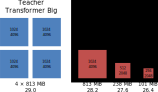
\includegraphics[width=0.9\textwidth]{teacher2.pdf}}

\vspace{3mm}
(Scale preserving)
\end{figure}
\end{frame}

% first column
\begin{frame}{}
\hfill%
\begin{tikzpicture}\small
\begin{axis}[xmajorgrids,
    width=0.9\textwidth,
    height=0.9\textheight,
    nodes near coords xbar stacked configuration/.style={},
    xbar stacked, y dir=reverse,
	bar width=15pt, ymin=0.5, ymax=8.5,xmin=0, xmax=550,
    enlargelimits=0.15,
    legend style={at={(0.5,1.05)}, anchor=north,legend columns=-1},
    xlabel={Seconds to translate newstest2014 (batch-size: ca.~384 words -- 5 to 25 sentences)},
    ytick={1,2,3,4,5,6,7.5,8.5},
    yticklabel style={align=right},
    yticklabels={Transformer-base, +Shortlist, +AAN (modified), +MM-int16, +Memoization, +Auto-tuning, {+Caching att.\\keys/values},{w/o \texttt{--optimize}}}
]
% MKL
\addplot+[xbar, bblue] coordinates {(479.8,1)}; 
% 16int-GEMM
\addplot+[xbar, rred] coordinates {(0,1) };
% Quant
\addplot+[xbar, oorange] coordinates {(0,1) };
  % Rest
\addplot+[xbar,lightgray,nodes near coords,every node near coord/.append style={black},/pgf/number format/fixed zerofill,/pgf/number format/precision=1] coordinates {(62.8,1) };
\legend{\strut MM-MKL, \strut MM-int16, \strut Quant-int16, \strut Other}
\end{axis}
\end{tikzpicture}
\end{frame}

\begin{frame}{}
\begin{figure}
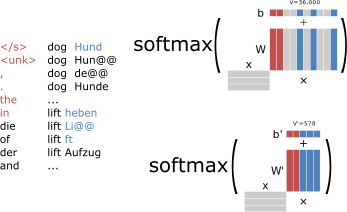
\includegraphics[width=0.9\textwidth]{shortlist.pdf}
\end{figure}
\end{frame}

% second column - shortlist
\begin{frame}{}
\centering
\begin{tikzpicture}\small
\begin{axis}[xmajorgrids,
    width=0.9\textwidth,
    height=0.9\textheight,
    nodes near coords xbar stacked configuration/.style={},
    xbar stacked, y dir=reverse,
	bar width=15pt, ymin=0.5, ymax=8.5,xmin=0, xmax=550,
    enlargelimits=0.15,
    legend style={at={(0.5,1.05)}, anchor=north,legend columns=-1},
    xlabel={Seconds to translate newstest2014 (batch-size: ca.~384 words -- 5 to 25 sentences)},
    ytick={1,2,3,4,5,6,7.5,8.5},
    yticklabel style={align=right},
    yticklabels={Transformer-base, +Shortlist, +AAN (modified), +MM-int16, +Memoization, +Auto-tuning, {+Caching att.\\keys/values},{w/o \texttt{--optimize}}}
]
% MKL
\addplot+[xbar, bblue] coordinates {(479.8,1) (351.3,2)}; 
% 16int-GEMM
\addplot+[xbar, rred] coordinates {(0,1) (0,2) };
% Quant
\addplot+[xbar, oorange] coordinates {(0,1) (0,2)};
  % Rest
\addplot+[xbar,lightgray,nodes near coords,every node near coord/.append style={black},/pgf/number format/fixed zerofill,/pgf/number format/precision=1] coordinates {(62.8,1) (60.7,2)  };

\legend{\strut MM-MKL, \strut MM-int16, \strut Quant-int16, \strut Other}
\end{axis}
\end{tikzpicture}
\end{frame}

\begin{frame}{}
\begin{columns}
\begin{column}[t]{0.45\textwidth}
Multiplicative attention:
\begin{eqnarray*}
Q'&=& QW_q + b_q \\
K' &=& KW_k + b_k \\
V' &=& VW_v + b_v \\
C &=& \mathrm{softmax}(Q'\times\Trans{(K')}) \times V' \\
Y &=& \mathrm{norm}(Q + C)
\end{eqnarray*}
\begin{itemize}
\item During training: $ Q = K = V $
\item During translation: $ Q \neq K; K = V $
\item Complexity per step: $O(n)$
\item Because: $c_t = \mathrm{softmax}(q'_t \times \Trans{(K'_{<t})})\times V'_{<t}$\\
$K_{<t+1} = [K_{<t} ; q_t]$
\end{itemize}\vfill
\end{column}
\hspace{-1cm} \pause
\begin{column}[t]{0.45\textwidth}
Average attention network\\ (Zhang et al. 2018):
\begin{eqnarray*}
C &=& \mathrm{gate}(\mathrm{FFN}(\bar{V}), Q) \\
Y &=& \mathrm{norm}(Q + C)
\end{eqnarray*}
\begin{itemize}
\item Gate and FFN optional
\item Complexity per step: $O(1)$
\item Because: $\bar{v}_t = \frac{1}{t}((t-1)\bar{v}_{t-1} + v_t)$
\item Basically a weird RNN
\item Authors report 4x speed-up for beam=4
\end{itemize}\vfill
\end{column}
\end{columns}
\end{frame}

% third column - AAN
\begin{frame}{}
\hfill%
\begin{tikzpicture}\small
\begin{axis}[xmajorgrids,
    width=0.9\textwidth,
    height=0.9\textheight,
    nodes near coords xbar stacked configuration/.style={},
    xbar stacked, y dir=reverse,
	bar width=15pt, ymin=0.5, ymax=8.5,xmin=0, xmax=550,
    enlargelimits=0.15,
    legend style={at={(0.5,1.05)}, anchor=north,legend columns=-1},
    xlabel={Seconds to translate newstest2014 (batch-size: ca.~384 words -- 5 to 25 sentences)},
    ytick={1,2,3,4,5,6,7.5,8.5},
    yticklabel style={align=right},
    yticklabels={Transformer-base, +Shortlist, +AAN (modified), +MM-int16, +Memoization, +Auto-tuning, {+Caching att.\\keys/values},{w/o \texttt{--optimize}}}
]
% MKL
\addplot+[xbar, bblue] coordinates {(479.8,1) (351.3,2) (262.4,3)}; 
% 16int-GEMM
\addplot+[xbar, rred] coordinates {(0,1) (0,2) (0,3)};
% Quant
\addplot+[xbar, oorange] coordinates {(0,1) (0,2) (0,3)};
  % Rest
\addplot+[xbar,lightgray,nodes near coords,every node near coord/.append style={black},/pgf/number format/fixed zerofill,/pgf/number format/precision=1] coordinates {(62.8,1) (60.7,2) (42.3,3) };

\legend{\strut MM-MKL, \strut MM-int16, \strut Quant-int16, \strut Other}
\end{axis}
\end{tikzpicture}
\end{frame}

% \newcommand{\todo}[1]{\textcolor{red}{#1}}
% \newcommand{\dotint}[2]{\mathrm{dot^{\prime}_{int}}(#1, #2)}
% \newcommand{\dotn}[3]{\mathrm{dot^{\prime}_{#1}}(#2, #3)}
% \newcommand{\quant}[1]{\mathrm{quant_{int}}(#1)}
% \newcommand{\Trans}[1]{#1^\mathrm{T}}

\begin{frame}{}

Code based on Devlin (2017), extended to AVX512

\centering\Large
\begin{eqnarray*}
\quant{x} &=& \mathrm{int16}(x \cdot 2^{10})\\ \pause
A_{\mathrm{q}} \otimes B_{\mathrm{q}} &=& A_{\mathrm{q}}\times \Trans{B_{\mathrm{q}}}  \\[10mm]
\pause
x \times W & = & x \times \Trans{(\Trans{W})} \\ 
           & \approx & \dotint{\quant{x}}{\quant{\Trans{W}}} \\
           & = & \quant{x} \otimes \quant{\Trans{W}} \\[5mm]
\end{eqnarray*}
\end{frame}

\begin{frame}{}
\centering
\resizebox{!}{8cm}{%
\begin{tikzpicture}[
    scale = 1.5, transform shape, thick,
    every node/.style = {draw, shape = rectangle, rounded corners, minimum size = 10mm}, grow = down, sibling distance=2cm]
\begin{scope}
  \node[fill=bblue!60] (root1) {\textrm{dot}$(x,W)$} 
  child { node[fill=bblue!60] (prod1) { $\times$ }
   child {   node [] (x1) {$x$} }
   child {   node [] (w1) {$W$} }
  };
  
  \invisible<1>{%
  \begin{scope}[nodes = {draw=none, right=30pt}]
      \node (measure3) at (prod1) {measure($h_1$)};
      \draw [->] (measure3) -- (prod1);
  \end{scope}}
\end{scope}
\begin{scope}[xshift=7cm]
  \node[fill=rred!60] (root2) {\textrm{dot}$_{16}(x,W)$} 
  child { node[fill=rred!60] (prod2) { $\otimes$ }
   child { node [fill=oorange!60] (qx) {$\mathrm{quantize}$} child { node [] (x2) {$x$} } }
   child { node [fill=oorange!60] (qw) {$\mathrm{quantize}$} child { node [fill=lightgray!60] (tw) {$\mathrm{transpose}$} child { node [] (w2) {$W$} } } }
  };
  
  \invisible<1>{
    \begin{scope}[nodes = {draw=none, right=40pt}]
      \node (constant1) at (qw) {constant};
      \node (constant2) at (tw) {constant};
      \node (parameter1) at (w2) {parameter};
    \end{scope}
    \draw [->] (constant1) -- (qw);
    \draw [->] (constant2) -- (tw);
    \draw [->] (parameter1) -- (w2);
    
    \draw[rounded corners] ($(qw.north west) + (-0.2,0.2)$) rectangle ($(qw.south east) + (0.2,-3.2)$) node[draw=none,midway,above=60pt,anchor=south west] (mem) {memoized};}
    
    \invisible<1>{%
    \begin{scope}[nodes = {draw=none, left=30pt}]
      \node (measure1) at (prod2) {measure($h_2$)};
      \node (measure2) at (qx) {measure($h_2$)};
      \draw [->] (measure1) -- (prod2);
      \draw [->] (measure2) -- (qx);
    \end{scope}}
\end{scope}
\invisible<1>{%
\node (auto) at (3.5,1) {dot-tuned($x,W$)};
\draw [-] (root1) -- (auto);
\draw [-] (root2) -- (auto);
\draw [->] (measure1) -- (auto);
\draw [->] (measure2) -- (auto);
\draw [->] (measure3) -- (auto);}
\end{tikzpicture}}
\end{frame}


% fourth - MM-int16
\begin{frame}{}
\hfill%
\begin{tikzpicture}\small
\begin{axis}[xmajorgrids,
    width=0.9\textwidth,
    height=0.9\textheight,
    nodes near coords xbar stacked configuration/.style={},
    xbar stacked, y dir=reverse,
	bar width=15pt, ymin=0.5, ymax=8.5,xmin=0, xmax=550,
    enlargelimits=0.15,
    legend style={at={(0.5,1.05)}, anchor=north,legend columns=-1},
    xlabel={Seconds to translate newstest2014 (batch-size: ca.~384 words -- 5 to 25 sentences)},
    ytick={1,2,3,4,5,6,7.5,8.5},
    yticklabel style={align=right},
    yticklabels={Transformer-base, +Shortlist, +AAN (modified), +MM-int16, +Memoization, +Auto-tuning, {+Caching att.\\keys/values},{w/o \texttt{--optimize}}}
]
% MKL
\addplot+[xbar, bblue] coordinates {(479.8,1) (351.3,2) (262.4,3) (4.1,4) }; 
% 16int-GEMM
\addplot+[xbar, rred] coordinates {(0,1) (0,2) (0,3) (227.4,4) };
% Quant
\addplot+[xbar, oorange] coordinates {(0,1) (0,2) (0,3) (47.7,4) };
  % Rest
\addplot+[xbar,lightgray,nodes near coords,every node near coord/.append style={black},/pgf/number format/fixed zerofill,/pgf/number format/precision=1] coordinates {(62.8,1) (60.7,2) (42.3,3) (226.7,4)};


\legend{\strut MM-MKL, \strut MM-int16, \strut Quant-int16, \strut Other}
\end{axis}
\end{tikzpicture}
\end{frame}


\begin{frame}{}
\centering
\resizebox{!}{8cm}{%
\begin{tikzpicture}[
    scale = 1.5, transform shape, thick,
    every node/.style = {draw, shape = rectangle, rounded corners, minimum size = 10mm}, grow = down, sibling distance=2cm]
\begin{scope}
  \node[fill=bblue!60] (root1) {\textrm{dot}$(x,W)$} 
  child { node[fill=bblue!60] (prod1) { $\times$ }
   child {   node [] (x1) {$x$} }
   child {   node [] (w1) {$W$} }
  };
  
  \invisible<1-5>{%
  \begin{scope}[nodes = {draw=none, right=30pt}]
      \node (measure3) at (prod1) {measure($h_1$)};
      \draw [->] (measure3) -- (prod1);
  \end{scope}}
\end{scope}
\begin{scope}[xshift=7cm]
  \node[fill=rred!60] (root2) {\textrm{dot}$_{16}(x,W)$} 
  child { node[fill=rred!60] (prod2) { $\otimes$ }
   child { node [fill=oorange!60] (qx) {$\mathrm{quantize}$} child { node [] (x2) {$x$} } }
   child { node [fill=oorange!60] (qw) {$\mathrm{quantize}$} child { node [fill=lightgray!60] (tw) {$\mathrm{transpose}$} child { node [] (w2) {$W$} } } }
  };
  
    \begin{scope}[nodes = {draw=none, right=40pt}]
      \uncover<4->{
      \node (constant1) at (qw) {$\mathrm{constant}$};
      \draw [->] (constant1) -- (qw);}
      
      \uncover<3->{
      \node (constant2) at (tw) {$\mathrm{constant}$};
      \draw [->] (constant2) -- (tw);}
      
      \uncover<2->{
      \node (parameter1) at (w2) {$\mathrm{parameter}$};
      \draw [->] (parameter1) -- (w2);}
    \end{scope}
    
    \uncover<5>{
    \draw[rounded corners] ($(qw.north west) + (-0.2,0.2)$) rectangle ($(qw.south east) + (0.2,-3.2)$) node[draw=none,midway,above=60pt,anchor=south west] (mem) {$\mathrm{memoized}$};}
    
    \invisible<1-5>{%
    \begin{scope}[nodes = {draw=none, left=30pt}]
      \node (measure1) at (prod2) {measure($h_2$)};
      \node (measure2) at (qx) {measure($h_2$)};
      \draw [->] (measure1) -- (prod2);
      \draw [->] (measure2) -- (qx);
    \end{scope}}
\end{scope}
\invisible<1-5>{%
\node (auto) at (3.5,1) {$\mathrm{dot-tuned}(x,W)$};
\draw [-] (root1) -- (auto);
\draw [-] (root2) -- (auto);
\draw [->] (measure1) -- (auto);
\draw [->] (measure2) -- (auto);
\draw [->] (measure3) -- (auto);}
\end{tikzpicture}}
\end{frame}

% fifth - memo
\begin{frame}{}
\hfill%
\begin{tikzpicture}\small
\begin{axis}[xmajorgrids,
    width=0.9\textwidth,
    height=0.9\textheight,
    nodes near coords xbar stacked configuration/.style={},
    xbar stacked, y dir=reverse,
	bar width=15pt, ymin=0.5, ymax=8.5,xmin=0, xmax=550,
    enlargelimits=0.15,
    legend style={at={(0.5,1.05)}, anchor=north,legend columns=-1},
    xlabel={Seconds to translate newstest2014 (batch-size: ca.~384 words -- 5 to 25 sentences)},
    ytick={1,2,3,4,5,6,7.5,8.5},
    yticklabel style={align=right},
    yticklabels={Transformer-base, +Shortlist, +AAN (modified), +MM-int16, +Memoization, +Auto-tuning, {+Caching att.\\keys/values},{w/o \texttt{--optimize}}}
]
% MKL
\addplot+[xbar, bblue] coordinates {(479.8,1) (351.3,2) (262.4,3) (4.1,4) (3.7,5) }; 
% 16int-GEMM
\addplot+[xbar, rred] coordinates {(0,1) (0,2) (0,3) (227.4,4) (251.2,5) };
% Quant
\addplot+[xbar, oorange] coordinates {(0,1) (0,2) (0,3) (47.7,4) (15.0,5)};
  % Rest
\addplot+[xbar,lightgray,nodes near coords,every node near coord/.append style={black},/pgf/number format/fixed zerofill,/pgf/number format/precision=1] coordinates {(62.8,1) (60.7,2) (42.3,3) (226.7,4) (44.4,5)};

\legend{\strut MM-MKL, \strut MM-int16, \strut Quant-int16, \strut Other}
\end{axis}
\end{tikzpicture}
\end{frame}


\begin{frame}{}
\centering
\resizebox{!}{8cm}{%
\begin{tikzpicture}[
    scale = 1.5, transform shape, thick,
    every node/.style = {draw, shape = rectangle, rounded corners, minimum size = 10mm}, grow = down, sibling distance=2cm]
\begin{scope}
  \node[fill=bblue!60] (root1) {\textrm{dot}$(x,W)$} 
  child { node[fill=bblue!60] (prod1) { $\times$ }
   child {   node [] (x1) {$x$} }
   child {   node [] (w1) {$W$} }
  };
  
  \invisible<1-2>{%
  \begin{scope}[nodes = {draw=none, right=30pt}]
      \node (measure3) at (prod1) {measure($h_1$)};
      \draw [->] (measure3) -- (prod1);
  \end{scope}}
\end{scope}
\begin{scope}[xshift=7cm]
  \node[fill=rred!60] (root2) {\textrm{dot}$_{16}(x,W)$} 
  child { node[fill=rred!60] (prod2) { $\otimes$ }
   child { node [fill=oorange!60] (qx) {$\mathrm{quantize}$} child { node [] (x2) {$x$} } }
   child { node [fill=oorange!60] (qw) {$\mathrm{quantize}$} child { node [fill=lightgray!60] (tw) {$\mathrm{transpose}$} child { node [] (w2) {$W$} } } }
  };
  
    \begin{scope}[nodes = {draw=none, right=40pt}]
      \node (constant1) at (qw) {$\mathrm{constant}$};
      \draw [->] (constant1) -- (qw);
      
      \node (constant2) at (tw) {$\mathrm{constant}$};
      \draw [->] (constant2) -- (tw);
      
      \node (parameter1) at (w2) {$\mathrm{parameter}$};
      \draw [->] (parameter1) -- (w2);
    \end{scope}
    
    \draw[rounded corners] ($(qw.north west) + (-0.2,0.2)$) rectangle ($(qw.south east) + (0.2,-3.2)$) node[draw=none,midway,above=60pt,anchor=south west] (mem) {$\mathrm{memoized}$};
    
    \invisible<1-2>{%
    \begin{scope}[nodes = {draw=none, left=30pt}]
      \node (measure1) at (prod2) {measure($h_2$)};
      \node (measure2) at (qx) {measure($h_2$)};
      \draw [->] (measure1) -- (prod2);
      \draw [->] (measure2) -- (qx);
    \end{scope}}
\end{scope}
\uncover<2>{%
\node (auto) at (3.5,1) {$\mathrm{autotune}(x,W)$};
\draw [-] (root1) -- (auto);
\draw [-] (root2) -- (auto);}
\invisible<1-2>{%
\draw [->] (measure1) -- (auto);
\draw [->] (measure2) -- (auto);
\draw [->] (measure3) -- (auto);}
\end{tikzpicture}}
\end{frame}

\begin{frame}{}
\begin{eqnarray*}
h_1 &=& \mathrm{hash}(\mathrm{dot}(x,W))\\
 &=& \mathrm{hash}(\mathrm{dot}) \odot \mathrm{hash}(\mathrm{dims}(x)) \odot \mathrm{hash}(\mathrm{dims}(W))\\
 &=& \mathrm{hash}(\mathrm{dot}) \odot \mathrm{hash}(\{11,512\}) \odot \mathrm{hash}(\{512,512\}) \\[5mm]
h_2 &=& \mathrm{hash}(\mathrm{dot_{16}}(x,W))\\
 &=& \mathrm{hash}(\mathrm{dot_{16}}) \odot \mathrm{hash}(\mathrm{dims}(x)) \odot \mathrm{hash}(\mathrm{dims}(W))\\
 &=& \mathrm{hash}(\mathrm{dot_{16}}) \odot \mathrm{hash}(\{11,512\}) \odot \mathrm{hash}(\{512,512\})
\end{eqnarray*}

\vspace{5mm}

We can decrease granularity via integer-dividing dimensions by a given factor, we choose 5. 
\end{frame}

\begin{frame}{}
\centering
\resizebox{!}{8cm}{%
\begin{tikzpicture}[
    scale = 1.5, transform shape, thick,
    every node/.style = {draw, shape = rectangle, rounded corners, minimum size = 10mm}, grow = down, sibling distance=2cm]
\begin{scope}
  \node[fill=bblue!60] (root1) {\textrm{dot}$(x,W)$} 
  child { node[fill=bblue!60] (prod1) { $\times$ }
   child {   node [] (x1) {$x$} }
   child {   node [] (w1) {$W$} }
  };
  
  \uncover<2>{%
  \begin{scope}[nodes = {draw=none, right=30pt}]
      \node (measure3) at (prod1) {$\mathrm{measure(h_1)}$};
      \draw [->] (measure3) -- (prod1);
  \end{scope}}
\end{scope}
\begin{scope}[xshift=7cm]
  \node[fill=rred!60] (root2) {\textrm{dot}$_{16}(x,W)$} 
  child { node[fill=rred!60] (prod2) { $\otimes$ }
   child { node [fill=oorange!60] (qx) {$\mathrm{quantize}$} child { node [] (x2) {$x$} } }
   child { node [fill=oorange!60] (qw) {$\mathrm{quantize}$} child { node [fill=lightgray!60] (tw) {$\mathrm{transpose}$} child { node [] (w2) {$W$} } } }
  };
  
    \begin{scope}[nodes = {draw=none, right=40pt}]
      \node (constant1) at (qw) {$\mathrm{constant}$};
      \draw [->] (constant1) -- (qw);
      
      \node (constant2) at (tw) {$\mathrm{constant}$};
      \draw [->] (constant2) -- (tw);
      
      \node (parameter1) at (w2) {$\mathrm{parameter}$};
      \draw [->] (parameter1) -- (w2);
    \end{scope}
    
    \draw[rounded corners] ($(qw.north west) + (-0.2,0.2)$) rectangle ($(qw.south east) + (0.2,-3.2)$) node[draw=none,midway,above=60pt,anchor=south west] (mem) {$\mathrm{memoized}$};
    
    \uncover<2>{%
    \begin{scope}[nodes = {draw=none, left=30pt}]
      \node (measure1) at (prod2) {$\mathrm{measure(h_2)}$};
      \node (measure2) at (qx) {$\mathrm{measure(h_2)}$};
      \draw [->] (measure1) -- (prod2);
      \draw [->] (measure2) -- (qx);
    \end{scope}}
\end{scope}
\node (auto) at (3.5,1) {$\mathrm{autotune(x,W)}$};
\draw [-] (root1) -- (auto);
\draw [-] (root2) -- (auto);
\uncover<2>{%
\draw [->] (measure1) -- (auto);
\draw [->] (measure2) -- (auto);
\draw [->] (measure3) -- (auto);}
\end{tikzpicture}}
\end{frame}


% sixth - auto
\begin{frame}{}
\hfill%
\begin{tikzpicture}\small
\begin{axis}[xmajorgrids,
    width=0.9\textwidth,
    height=0.9\textheight,
    nodes near coords xbar stacked configuration/.style={},
    xbar stacked, y dir=reverse,
	bar width=15pt, ymin=0.5, ymax=8.5,xmin=0, xmax=550,
    enlargelimits=0.15,
    legend style={at={(0.5,1.05)}, anchor=north,legend columns=-1},
    xlabel={Seconds to translate newstest2014 (batch-size: ca.~384 words -- 5 to 25 sentences)},
    ytick={1,2,3,4,5,6,7.5,8.5},
    yticklabel style={align=right},
    yticklabels={Transformer-base, +Shortlist, +AAN (modified), +MM-int16, +Memoization, +Auto-tuning, {+Caching att.\\keys/values},{w/o \texttt{--optimize}}}
]
% MKL
\addplot+[xbar, bblue] coordinates {(479.8,1) (351.3,2) (262.4,3) (4.1,4) (3.7,5) (130.9,6) }; 
% 16int-GEMM
\addplot+[xbar, rred] coordinates {(0,1) (0,2) (0,3) (227.4,4) (251.2,5) (94.6,6)};
% Quant
\addplot+[xbar, oorange] coordinates {(0,1) (0,2) (0,3) (47.7,4) (15.0,5) (13.9,6)};
  % Rest
\addplot+[xbar,lightgray,nodes near coords,every node near coord/.append style={black},/pgf/number format/fixed zerofill,/pgf/number format/precision=1] coordinates {(62.8,1) (60.7,2) (42.3,3) (226.7,4) (44.4,5) (42.5,6) };

\only<2>{\draw [decorate,decoration={brace,amplitude=5pt,mirror},xshift=-0.5em]
(0.5,3.5) -- (0.5,6.5) node [black,midway,xshift=-1em,rotate=90] {\texttt{--optimize}};}

\legend{\strut MM-MKL, \strut MM-int16, \strut Quant-int16, \strut Other}
\end{axis}
\end{tikzpicture}
\end{frame}

% full graph
\begin{frame}{}
\hfill%
\begin{tikzpicture}\small
\begin{axis}[xmajorgrids,
    width=0.9\textwidth,
    height=0.9\textheight,
    nodes near coords xbar stacked configuration/.style={},
    xbar stacked, y dir=reverse,
	bar width=15pt, ymin=0.5, ymax=8.5,xmin=0, xmax=550,
    enlargelimits=0.15,
    legend style={at={(0.5,1.05)}, anchor=north,legend columns=-1},
    xlabel={Seconds to translate newstest2014 (batch-size: ca.~384 words -- 5 to 25 sentences)},
    ytick={1,2,3,4,5,6,7.5,8.5},
    yticklabel style={align=right},
    yticklabels={Transformer-base, +Shortlist, +AAN (modified), +MM-int16, +Memoization, +Auto-tuning, {+Caching att.\\keys/values},{w/o \texttt{--optimize}}}
]
% MKL
\addplot+[xbar, bblue] coordinates {(479.8,1) (351.3,2) (262.4,3) (4.1,4) (3.7,5) (130.9,6) (21.8,7.5) (150.7,8.5)}; 
% 16int-GEMM
\addplot+[xbar, rred] coordinates {(0,1) (0,2) (0,3) (227.4,4) (251.2,5) (94.6,6) (85.8,7.5) (0,8.5)};
% Quant
\addplot+[xbar, oorange] coordinates {(0,1) (0,2) (0,3) (47.7,4) (15.0,5) (13.9,6) (15.2,7.5) (0,8.5)};
  % Rest
\addplot+[xbar,lightgray,nodes near coords,every node near coord/.append style={black},/pgf/number format/fixed zerofill,/pgf/number format/precision=1] coordinates {(62.8,1) (60.7,2) (42.3,3) (226.7,4) (44.4,5) (42.5,6) (34.2,7.5) (31.9,8.5) };

\draw [dashed] (-100,6.75) -- (650,6.75) node [below,near end] {Marian v1.5};

\draw [decorate,decoration={brace,amplitude=5pt,mirror},xshift=-0.5em]
(0.5,3.5) -- (0.5,6.5) node [black,midway,xshift=-1em,rotate=90] {\texttt{--optimize}}; 

\legend{\strut MM-MKL, \strut MM-int16, \strut Quant-int16, \strut Other}
\end{axis}
\end{tikzpicture}
\end{frame}

\begin{frame}{}
\centering
\begin{tikzpicture}\small
\begin{axis}[xmajorgrids,
    width=0.9\textwidth,
    height=0.7\textheight, xmin=0,
    nodes near coords xbar stacked configuration/.style={},
    xbar, y dir=reverse,
	bar width=15pt,
	nodes near coords,
    enlargelimits=0.15,
    legend style={at={(0.5,1.05)},
      anchor=north,legend columns=-1},
    xlabel={Latency per sentence in milliseconds for newstest2014 (batch-size: 1 sentence)},
    %symbolic y coords={Marian-v1.5,autotune,memoization,int16,AAN,shortlist,Transformer-base},
    ytick=data,
    yticklabel style={align=right},
    yticklabels={Transformer-base, +Shortlist, +AAN (modified), using \texttt{--optimize}, {+Caching att.\\keys/values},{w/o \texttt{--optimize}}}
]
    
% ALL
\addplot+[xbar, bblue,
nodes near coords,
every node near coord/.append style={black},
/pgf/number format/fixed zerofill,
/pgf/number format/precision=1] coordinates {
(1371.91/2737*1000,1) (942.9/2737*1000,2) (726.4/2737*1000,3) (554.9/2737*1000,4) (364.1/2737*1000,5.5) %64(364.1/2737*1000,6.5) 
(588.8/2737*1000,6.5)
};
 
\draw [dashed] (-100,4.75) -- (600,4.75) node [below,near end] {Marian v1.5};

\end{axis}
\end{tikzpicture}
\end{frame}

% % mkl 1.5 - 
% % all 1.5 - 151.2

% \begin{frame}{}
% \begin{table}
% \centering\renewcommand{\arraystretch}{0.95}
% \begin{tabular}{cp{7cm}rrrr}
% \toprule
% No & Model & MiB & Time & (v1.5) & BLEU \\
% \midrule
% (1) & Baseline GPU & -- & 51.6 &  & 16.8\\
% (2) & Sockeye GPU (Transformer-base b=5) &  & 231.9 &  & 27.6 \\
% \midrule
% %& Teacher - Transformer-big b=4 & 813 & 75.5 & 28.2 \\
% (3) & Teacher - Transformer-big b=8 & 813 & 109.7 & -- & 28.1 \\
% (4) & Teacher - Transformer-big$\times 4$ b=8 & 3252 & 410.8 & (211.1) & 29.0 \\
% \midrule
% (6) & Transformer-big b=2 &  813 &  31.9 & (15.4) & 28.4 \\ %ok
% (12) & Transformer-base-AAN b=2 & 220 & 8.9 & (6.5) & 27.7 \\
% (16) & Transformer-small-AAN -ffn &  98 & 5.7 & (4.6) & 26.2 \\
% (18) &  RNN-small-Amun &  88 & 1.6 & -- & 24.1 \\ % ok
% \bottomrule
% \end{tabular}
% \caption{GPU baselines, teachers and submitted systems}
% \end{table}
% \end{frame}

% \begin{frame}{}
% \begin{table}
% \resizebox{9cm}{!}{%
% \centering\renewcommand{\arraystretch}{0.95}
% \begin{tabular}{cp{7cm}rrrr}
% \toprule
% No & Model & MiB & Time & (v1.5) & BLEU \\
% \midrule
% (1) & Baseline GPU & -- & 51.6 & & 16.8\\
% (2) & Sockeye GPU (Transformer-base b=5) & -- & 231.9 & & 27.6 \\
% \midrule
% %& Teacher - Transformer-big b=4 & 813 & 75.5 & 28.2 \\
% (3) & Teacher - Transformer-big b=8 & 813 & 109.7 & -- & 28.1 \\
% (4) & Teacher - Transformer-big$\times 4$ b=8 & 3252 & 410.8 & (211.1) & 29.0 \\
% \midrule
% (5) & Transformer-big b=4 & 813 & 52.0 & -- & 28.4 \\ % ok
% (6) & \bf Transformer-big b=2 & \bf 813 & \bf 31.9 & \bf (15.4) & \bf 28.4 \\ %ok
% (7) & Transformer-big & 813 & 19.9 & -- & 28.2 \\  \midrule %ok
% (8) & Transformer-base b=4 & 238 & 40.5 & -- & 27.8 \\ % ok
% (9) & Transformer-base b=2 & 238 & 22.9 & -- & 27.8 \\ % ok
% (10) & Transformer-base & 238 & 12.8 & -- & 27.6 \\ \midrule % ok
% (11) & Transformer-base-AAN b=4 & 220 & 15.9 & -- & 27.7 \\
% (12) & \bf Transformer-base-AAN b=2 &\bf 220 &\bf 8.9 & \bf (6.5) &\bf 27.7 \\
% (13) & Transformer-base-AAN & 220 & 7.2 & -- &  27.6 \\ \midrule
% (14) & Transformer-small & 101 & 10.8 & -- & 26.4 \\ \midrule
% (15) & Transformer-small-AAN & 100 & 5.9 & -- & 25.8 \\
% (16) & \bf Transformer-small-AAN -ffn & \bf 98 & \bf 5.7 & \bf (4.6) & \bf 26.2 \\
% (17) & Transformer-small-AAN -ffn -gate & 95 & 5.6 & -- & 25.8 \\ \midrule
% (18) & \bf RNN-small-Amun & \bf 88 & \bf 1.6 & \bf -- & \bf  24.1 \\ % ok
% (19) & RNN-Nematus-Amun & 199 & 2.2 & -- & 24.8 \\ \midrule %ok
% (20) & RNN-small& 88 & 1.8 & -- & 24.1 \\ % ok
% (21) & RNN-Nematus & 199 & 2.5 & -- & 24.8 \\ % ok
% (22) & RNN-Deep & 323 & 2.9 & -- & 25.7 \\ %ok
% \bottomrule
% \end{tabular}}
% \caption{All GPU systems explored in this work}
% \end{table}
% \end{frame}

% \begin{frame}{}
% \begin{table}
% \centering\renewcommand{\arraystretch}{0.95}
% \begin{tabular}{cp{7cm}rrrr}
% \toprule
% No & Model & MiB & Time & (v1.5) & BLEU \\
% \midrule
% (1) & Baseline CPU & -- & 4492.2 & & 16.8 \\
% (2) & Sockeye CPU (Transformer-base b=5) & -- & 1168.6 &  & 27.4 \\ \midrule
% (7) &  Transformer-big & 813 & 1537.8 & (1037.1) & 28.1 \\
% (7i) & Transformer-big-int8 & 813 &  1169.9 & -- &  27.5 \\ \midrule
% (13i) & Transformer-base-AAN-int16 & 220 & 273.2 & (159.5) &  27.5 \\ \midrule
% (17i) & Transformer-small-AAN-int16 -ffn -gate &  95 &  94.1 & (62.2) &  26.0 \\ \midrule
% (23i) & Transformer-tiny-256-AAN-int16 -ffn -gate* & 84 & 79.7 & (56.6) & 25.3 \\
% (24i) & Transformer-tiny-192-AAN-int16 -ffn -gate* & 60 & 61.1 & (42.3) & 24.4 \\
% \bottomrule
% \end{tabular}
% \caption{CPU baselines and submitted systems}
% \end{table}
% \end{frame}

% \begin{frame}{}
% \begin{table}
% \resizebox{9cm}{!}{%
% \centering\renewcommand{\arraystretch}{0.95}
% \begin{tabular}{cp{7cm}rrrr}
% \toprule
% No & Model & MiB & Time & (v1.5) & BLEU \\
% \midrule
% (1) & Baseline CPU & -- & 4492.2 &  & 16.8 \\
% (2) & Sockeye CPU (Transformer-base b=5) & -- & 1168.6 & & 27.4 \\ \midrule
% (7) & \bf Transformer-big & \bf 813 & \bf 1537.8 & \bf (1037.1) & \bf 28.1 \\
% (7i) & \bf Transformer-big-int8 & \bf 813 & \bf 1169.9 & \bf -- & \bf 27.5 \\ \midrule
% (10) & Transformer-base & 238 & 393.1 & -- & 27.4 \\
% (10i) & Transformer-base-int16 & 238 & 400.2 & -- & 27.4 \\ \midrule
% (13) & Transformer-base-AAN & 220 & 288.7 & -- &  27.5 \\
% (13i) & \bf Transformer-base-AAN-int16 & \bf 220 & \bf 273.2 & \bf (159.5) & \bf 27.5 \\ \midrule
% (14) & Transformer-small & 101 & 134.1 & -- & 26.5 \\  
% (14i) & Transformer-small-int16 & 101 & 133.2 & -- & 26.5 \\  \midrule
% (15i) & Transformer-small-AAN-int16 & 100 & 108.8 & -- & 25.8 \\
% (16i) & Transformer-small-AAN-int16 -ffn  & 98 & 108.3 & -- & 26.2 \\
% (17) & Transformer-small-AAN -ffn -gate & 95 & 100.6 & -- & 26.0 \\
% (17i) & \bf Transformer-small-AAN-int16 -ffn -gate & \bf 95 & \bf 94.1 & \bf (62.2) & \bf 26.0 \\ \midrule
% (23i) & Transformer-tiny-256-AAN-int16 -ffn -gate* & 84 & 79.7 & (56.6) & 25.3 \\
% (24i) & Transformer-tiny-192-AAN-int16 -ffn -gate* & 60 & 61.1 & (42.3) & 24.4 \\
% \bottomrule
% \end{tabular}}
% \caption{All CPU systems explored in this work}
% \end{table}
% \end{frame}

\begin{frame}{}

\centering
Map GPU and CPU performance into comparable space [w/\$] \\[5mm]

newstest2014.de consists of 62,954 tokens
\vspace{0.5cm}

\begin{table}
\begin{tabular}{lc} \toprule
Type & Price [\$/h] \\ \midrule
p3.x2large & 3.259 \\
m5.large & 0.102 \\ \bottomrule
\end{tabular}
\end{table}\vspace{0.5cm}

$$ [\mathrm{w}/\$] = \frac{62,954\;\mathrm{[w]}}{\mathrm{Translation\;time\;[s]}} \cdot \frac{3,600\;\mathrm{\left[s/h\right]}}{\mathrm{Instance\; price\;\left[\$/h\right]}}. $$

\end{frame}

\begin{frame}{}
\begin{figure}
\centering
\resizebox{11cm}{!}{%
\begin{tikzpicture}
\begin{axis}[
scale=.95,
xmode=log,
xmin=0.08, xmax=125,
xtick={0.1, 1, 10, 100},
log ticks with fixed point,
every non boxed x axis/.style={}, 
scale only axis,
ymajorgrids, yminorgrids=false,
xmajorgrids, xminorgrids,
x axis line style=-,
group style={
group name=break2,
group size=1 by 2,
xticklabels at=edge bottom,
vertical sep=0pt
},
minor grid style={gray!30, ultra thin},
y tick label style={/pgf/number format/fixed,
/pgf/number format/fixed zerofill,
/pgf/number format/precision=1},
xtick distance=5,
visualization depends on={value \thisrow{sysid} \as \thesystem},
nodes near coords=\thesystem,
every node near coord/.append style={anchor=north, font=\scriptsize, xshift=0pt},
legend columns=2, 
legend style={at={(0.5,1.07)},anchor=north,font=\small, /tikz/column 2/.style={column sep=5pt},},
%legend style={at={(0.3,.3)},anchor=north,font=\small, /tikz/column 2/.style={column sep=5pt},},
width=14cm,
height=10cm,
ymin=16.0, ymax=30.5,
restrict y to domain=16.5:29.5,
ylabel={BLEU}, xlabel={Million translated source tokens per USD (log scale)},
]

\only<2,5>{
\addplot [only marks, bblue, mark=x, very thick, mark size=3]
table[x expr={62954 / \thisrow{time} * 3600/3.259 / 10^6}, y=bleu] {gpu.systems.marian};}

\only<4,5>{
\addplot [only marks, rred, mark=x, very thick, mark size=3]
table[x expr={62954 / \thisrow{timed} * 3600/0.102 / 10^6}, y=bleu] {cpu.systems.marian};}

\only<1,2,5>{
\addplot [only marks, bblue, mark=o, very thick, mark size=3]
table[x expr={62954 / \thisrow{time} * 3600/3.259 / 10^6}, y=bleu] {gpu.systems.other};}

\only<3,4,5>{
\addplot [only marks, rred, mark=o, very thick, mark size=3]
table[x expr={62954 / \thisrow{time} * 3600/0.102 / 10^6}, y=bleu] {cpu.systems.other};}

\only<2,5>{
\addplot [only marks, black, mark=square, mark size=3, nodes near coords={}]
table[x expr={62954 / \thisrow{time} * 3600/3.259 / 10^6}, y=bleu] {gpu.systems.marian.submitted};}

\node at (axis cs:85,29.8) {\Cooley[1.5]};

\only<4,5>{
\addplot [only marks, black, mark=square, mark size=3, nodes near coords={}]
table[x expr={62954 / \thisrow{timed} * 3600/0.102 / 10^6}, y=bleu] {cpu.systems.marian.submitted};}

\only<3,4,5>{
\addplot [only marks, rred, mark=o, very thick, mark size=3, nodes near coords={}]
table[x expr={62954 / \thisrow{time} * 3600/0.102 / 10^6}, y=bleu] {cpu.systems.other2};}

\only<1,2,5>{
\addplot [only marks, bblue, mark=o, very thick, mark size=3, nodes near coords={}]
table[x expr={62954 / \thisrow{time} * 3600/3.259 / 10^6}, y=bleu] {gpu.systems.other2};}

\node at (axis cs:85,29.8) {\Cooley[1.5]};

\only<1>{\legend{Others GPU}}
\only<2>{\legend{Marian GPU, Others GPU, Submissions}}

\only<3>{\legend{Others CPU}}
\only<4>{\legend{Marian CPU, Others CPU, Submissions}}

\only<5>{\legend{Marian GPU, Marian CPU, Others GPU, Others CPU, Submissions}}
\end{axis}
\end{tikzpicture}}
\end{figure}
\end{frame}

\begin{frame}{}
\begin{figure}
\centering
\resizebox{11cm}{!}{%
\begin{tikzpicture}

\begin{axis}[
scale=.95,
xmode=log,
xmin=0.08, xmax=125,
xtick={0.1, 1, 10, 100},
log ticks with fixed point,
every non boxed x axis/.style={}, 
scale only axis,
ymajorgrids, yminorgrids=false,
xmajorgrids, xminorgrids,
x axis line style=-,
group style={
group name=break2,
group size=1 by 2,
xticklabels at=edge bottom,
vertical sep=0pt
},
minor grid style={gray!30, ultra thin},
y tick label style={/pgf/number format/fixed,
/pgf/number format/fixed zerofill,
/pgf/number format/precision=1},
xtick distance=5,
visualization depends on={value \thisrow{sysid} \as \thesystem},
legend columns=2, 
legend style={at={(0.5,1.07)},anchor=north,font=\small, /tikz/column 2/.style={column sep=5pt},},
%legend style={at={(0.3,.3)},anchor=north,font=\small, /tikz/column 2/.style={column sep=5pt},},
width=14cm,
height=10cm,
ymin=16.0, ymax=30.5,
restrict y to domain=16.5:29.5,
ylabel={BLEU}, xlabel={Million translated source tokens per USD (log scale)},
]

\only<1>{\addplot [bblue, smooth, very thick]
table[x expr={62954 / \thisrow{time} * 3600/3.259 / 10^6}, y=bleu] {gpu.systems.marian.line};}

\only<1>{
\addplot [rred, smooth, very thick]
 table[x expr={62954 / \thisrow{timed} * 3600/0.102 / 10^6}, y=bleu] {cpu.systems.marian.line};}

\only<2>{%
\addplot [bblue!40, smooth, very thick]
table[x expr={62954 / \thisrow{time} * 3600/3.259 / 10^6}, y=bleu] {gpu.systems.marian.line};
\addplot [rred!40, smooth, very thick]
 table[x expr={62954 / \thisrow{timed} * 3600/0.102 / 10^6}, y=bleu] {cpu.systems.marian.line};
}

\only<2>{%
\addplot [bblue, smooth, very thick]
table[x expr={62954 / \thisrow{time2} * 3600/3.259 / 10^6}, y=bleu] {gpu.systems.marian.line};
\addplot [rred, smooth, very thick]
 table[x expr={62954 / \thisrow{timed2} * 3600/0.102 / 10^6}, y=bleu] {cpu.systems.marian.line};}

\addplot [bblue, smooth, dashed, very thick]
table[x expr={62954 / \thisrow{time} * 3600/3.259 / 10^6}, y=bleu] {gpu.systems.other.line};

\addplot [rred, smooth, dashed, very thick]
 table[x expr={62954 / \thisrow{time} * 3600/0.102 / 10^6}, y=bleu] {cpu.systems.other.line};

\node at (axis cs:85,29.8) {\Cooley[1.5]};

\only<1>{\legend{Marian v1.4 GPU, Marian v1.4 CPU, Others GPU, Others CPU}}
\only<2>{\legend{Marian v1.4 GPU, Marian v1.4 CPU, Marian v1.5 GPU, Marian v1.5 CPU, Others GPU, Others CPU}}
\end{axis}
\end{tikzpicture}}
\end{figure}
\end{frame}

\begin{frame}{Future work}
\begin{itemize}
\item More experiments with Teacher-Student scenario;
\item More SIMD operations on the CPU;
\item All operations in fixed-point arithmetics on the CPU;
\item 8-bit matrix product on the CPU;
\item Mixed precision (FP16) on the GPU;
\item Optimize beam-search for batched translation;
\item ...
\end{itemize}
\end{frame}

{
\setbeamercolor{background canvas}{bg=}
\includepdf[pages=2]{acl.pdf}
}

\end{document}
